% answers.tex —— 2007 年·普通高等学校招生考试·湖南卷·理科 · 参考答案与详细解析片段
% 由 tools/generate_projects.py 依来源总账自 2007/2007_数学真题_湖南理_试题.md + 2007/2007_数学真题_湖南理_解析正文.md + 2007/2007_数学真题_湖南理_答案要点.md 生成，勿手改（改源 MD 后重跑）


\begin{gktip}
固定候选 PDF 仅含题面，无答案、解析和评分标准，原卷亦未标注分值；以下为非官方编者独立推导，官方答案字段为空。来源发布者、出版者、版次与官方身份均未核。
\end{gktip}

\begin{answer}
\gksolhead{1}{}

\textbf{题目}：

复数 $\left(\dfrac{2\mathrm i}{1+\mathrm i}\right)^2$ 等于（　）

（A）$4\mathrm i$

（B）$-4\mathrm i$

（C）$2\mathrm i$

（D）$-2\mathrm i$

\Needspace{4\baselineskip}
\textbf{解析}

\Needspace{5\baselineskip}
计算如下：

\nopagebreak[4]
\[\frac{2\mathrm i}{1+\mathrm i}=\frac{2\mathrm i(1-\mathrm i)}2=\mathrm i(1-\mathrm i)=1+\mathrm i,\]

\Needspace{5\baselineskip}
故

\nopagebreak[4]
\[\left(\frac{2\mathrm i}{1+\mathrm i}\right)^2=(1+\mathrm i)^2=2\mathrm i.\]

\gkanswer{答案：C。}

\end{answer}
\begin{answer}
\gksolhead{2}{}

\textbf{题目}：

不等式 $\dfrac{x-2}{x+1}\leqslant0$ 的解集是（　）

（A）$(-\infty,-1)\cup(-1,2]$

（B）$[-1,2]$

（C）$(-\infty,-1)\cup[2,+\infty)$

（D）$(-1,2]$

\Needspace{4\baselineskip}
\textbf{解析}

\Needspace{5\baselineskip}
$\dfrac{x-2}{x+1}\leqslant0$ 等价于 $(x-2)(x+1)\leqslant0$ 且 $x\neq-1$，即

\nopagebreak[4]
\[-1<x\leqslant2.\]

\gkanswer{答案：D。}

\end{answer}
\begin{answer}
\gksolhead{3}{}

\textbf{题目}：

设 $M$，$N$ 是两个集合，则“$M\cup N\neq\varnothing$”是“$M\cap N\neq\varnothing$”的（　）

（A）充分不必要条件

（B）必要不充分条件

（C）充分必要条件

（D）既不充分又不必要条件

\Needspace{4\baselineskip}
\textbf{解析}

$M\cap N\neq\varnothing$ 时 $M\cup N\neq\varnothing$，故必要性成立；取 $M=\{1\}$，$N=\{2\}$，则 $M\cup N\neq\varnothing$ 而 $M\cap N=\varnothing$，故充分性不成立。

\gkanswer{答案：B。}

\end{answer}
\begin{answer}
\gksolhead{4}{}

\textbf{题目}：

设 $\boldsymbol a$，$\boldsymbol b$ 是非零向量，若函数 $f(x)=(x\boldsymbol a+\boldsymbol b)\cdot(\boldsymbol a-x\boldsymbol b)$ 的图象是一条直线，则必有（　）

（A）$\boldsymbol a\perp\boldsymbol b$

（B）$\boldsymbol a\parallel\boldsymbol b$

（C）$|\boldsymbol a|=|\boldsymbol b|$

（D）$|\boldsymbol a|\neq|\boldsymbol b|$

\Needspace{4\baselineskip}
\textbf{解析}

\Needspace{5\baselineskip}
计算如下：

\nopagebreak[4]
\[f(x)=(x\boldsymbol a+\boldsymbol b)\cdot(\boldsymbol a-x\boldsymbol b)
=-(\boldsymbol a\cdot\boldsymbol b)x^2+\left(\boldsymbol a^2-\boldsymbol b^2\right)x+\boldsymbol a\cdot\boldsymbol b.\]

图象为直线，二次项系数必须为零，即 $\boldsymbol a\cdot\boldsymbol b=0$，故 $\boldsymbol a\perp\boldsymbol b$。

\gkanswer{答案：A。}

\end{answer}
\begin{answer}
\gksolhead{5}{}

\textbf{题目}：

设随机变量 $\xi$ 服从标准正态分布 $N(0,1)$。已知 $\Phi(-1.96)=0.025$，则 $P(|\xi|<1.96)=$（　）

（A）$0.025$

（B）$0.050$

（C）$0.950$

（D）$0.975$

\Needspace{4\baselineskip}
\textbf{解析}

\Needspace{5\baselineskip}
由标准正态分布的对称性，

\nopagebreak[4]
\[P(|\xi|<1.96)=1-2\Phi(-1.96)=1-2\times0.025=0.950.\]

\gkanswer{答案：C。}

\end{answer}
\begin{answer}
\gksolhead{6}{}

\textbf{题目}：

函数 $f(x)=\begin{cases}4x-4,&x\leqslant1,\\ x^2-4x+3,&x>1,\end{cases}$ 的图象和函数 $g(x)=\log_2x$ 的图象的交点个数是（　）

（A）$4$

（B）$3$

（C）$2$

（D）$1$

\Needspace{4\baselineskip}
\textbf{解析}

当 $x\leqslant1$ 时，$f(x)=4x-4$。$f(1)=g(1)=0$；在 $(0,1)$ 内 $4x-4=\log_2x$ 有且只有一个根（左端 $f-g>0$，在 $x=\dfrac12$ 处 $f-g=-1<0$，且 $f-g$ 在 $(0,1)$ 上单调递增）。

当 $x>1$ 时，$f(x)=(x-1)(x-3)$。$1<x<3$ 时 $f(x)<0<g(x)$，无交点；$x>3$ 时 $f(3)=0<g(3)$，$f(4)=3>g(4)=2$，有且只有一个交点。

共 $3$ 个交点。

\gkanswer{答案：B。}

\end{answer}
\begin{answer}
\gksolhead{7}{}

\textbf{题目}：

下列四个命题中，不正确的是（　）

（A）若函数 $f(x)$ 在 $x=x_0$ 处连续，则 $\lim\limits_{x\to x_0^+}f(x)=\lim\limits_{x\to x_0^-}f(x)$

（B）函数 $f(x)=\dfrac{x+2}{x^2-4}$ 的不连续点是 $x=2$ 和 $x=-2$

（C）若函数 $f(x)$，$g(x)$ 满足 $\lim\limits_{x\to\infty}[f(x)-g(x)]=0$，则 $\lim\limits_{x\to\infty}f(x)=\lim\limits_{x\to\infty}g(x)$

（D）$\lim\limits_{x\to1}\frac{\sqrt x-1}{x-1}=\frac12$

\Needspace{4\baselineskip}
\textbf{解析}

（A）连续的定义即左右极限存在且相等，正确。

（B）$f(x)=\dfrac{x+2}{(x-2)(x+2)}$，在 $x=\pm2$ 处无定义，正确。

（C）反例：$f(x)=x+\dfrac1x$，$g(x)=x$，则 $f(x)-g(x)=\dfrac1x\to0$（$x\to\infty$），但 $\lim\limits_{x\to\infty}f(x)$ 不存在，错误。

（D）$\dfrac{\sqrt x-1}{x-1}=\dfrac1{\sqrt x+1}\to\dfrac12$，正确。

\gkanswer{答案：C。}

\end{answer}
\begin{answer}
\gksolhead{8}{}

\textbf{题目}：

棱长为 $1$ 的正方体 $ABCD-A_1B_1C_1D_1$ 的 $8$ 个顶点都在球 $O$ 的表面上，$E$，$F$ 分别是棱 $AA_1$，$DD_1$ 的中点，则直线 $EF$ 被球 $O$ 截得的线段长为（　）

（A）$\frac{\sqrt2}2$

（B）$1$

（C）$1+\frac{\sqrt2}2$

（D）$\sqrt2$

\Needspace{4\baselineskip}
\textbf{解析}

\Needspace{5\baselineskip}
正方体外接球球心为正方体中心，半径

\nopagebreak[4]
\[R=\frac{\sqrt3}2.\]

$E$，$F$ 分别是 $AA_1$，$DD_1$ 的中点，故 $EF\parallel AD$，$EF=1$，且 $EF$ 到球心的距离为 $\dfrac12$（$EF$ 位于过棱 $AD$ 中点、垂直 $AD$ 的中截面内，到中心距离为底面半对角线的一半）。

\Needspace{5\baselineskip}
截得弦长

\nopagebreak[4]
\[2\sqrt{R^2-\left(\frac12\right)^2}=2\sqrt{\frac34-\frac14}=\sqrt2.\]

\gkanswer{答案：D。}

\end{answer}
\begin{answer}
\gksolhead{9}{}

\textbf{题目}：

设 $F_1$，$F_2$ 分别是椭圆 $\dfrac{x^2}{a^2}+\dfrac{y^2}{b^2}=1$（$a>b>0$）的左、右焦点，若在其右准线上存在 $P$，使线段 $PF_1$ 的中垂线过点 $F_2$，则椭圆离心率的取值范围是（　）

（A）$\left(0,\frac{\sqrt2}2\right]$

（B）$\left(0,\frac{\sqrt3}3\right]$

（C）$\left[\frac{\sqrt2}2,1\right)$

（D）$\left[\frac{\sqrt3}3,1\right)$

\Needspace{4\baselineskip}
\textbf{解析}

\Needspace{5\baselineskip}
设 $P\left(\dfrac{a^2}c,y\right)$。$PF_1$ 的中垂线过 $F_2$，等价于

\nopagebreak[4]
\[|PF_2|=|F_1F_2|=2c.\]

\Needspace{5\baselineskip}
于是

\nopagebreak[4]
\[\left(\frac{a^2}c-c\right)^2+y^2=4c^2,\]

\Needspace{5\baselineskip}
即

\nopagebreak[4]
\[y^2=4c^2-\frac{b^4}{c^2}.\]

\Needspace{5\baselineskip}
$P$ 存在要求 $y^2\geqslant0$：

\nopagebreak[4]
\[4c^4\geqslant b^4\ \Longrightarrow\ 2c^2\geqslant b^2=a^2-c^2\ \Longrightarrow\ 3c^2\geqslant a^2,\]

\Needspace{5\baselineskip}
故

\nopagebreak[4]
\[e^2\geqslant\frac13,\qquad e\geqslant\frac{\sqrt3}3.\]

又 $0<e<1$，故 $e\in\left[\dfrac{\sqrt3}3,1\right)$。

\gkanswer{答案：D。}

\end{answer}
\begin{answer}
\gksolhead{10}{}

\textbf{题目}：

设集合 $M=\{1,2,3,4,5,6\}$，$S_1$，$S_2$，$\cdots$，$S_k$ 都是 $M$ 的含两个元素的子集，且满足：对任意的 $S_i=\{a_i,b_i\}$，$S_j=\{a_j,b_j\}$（$i\neq j$，$i,j\in\{1,2,3,\cdots,k\}$），都有 $\min\left\{\dfrac{a_i}{b_i},\dfrac{b_i}{a_i}\right\}\neq\min\left\{\dfrac{a_j}{b_j},\dfrac{b_j}{a_j}\right\}$（$\min\{x,y\}$ 表示两个数 $x$，$y$ 中的较小者）。则 $k$ 的最大值是（　）

（A）$10$

（B）$11$

（C）$12$

（D）$13$

\Needspace{4\baselineskip}
\textbf{解析}

对二元子集 $\{a,b\}$（$a<b$），$\min\left\{\dfrac ab,\dfrac ba\right\}=\dfrac ab$。不同的 $\{a,b\}$ 可能给出相同的 $\dfrac ab$（如 $\{1,2\}$ 与 $\{2,4\}$），故 $k$ 的最大值等于 $\{1,2,\cdots,6\}$ 中互异比值 $\dfrac ab$（$a<b$，已约分）的个数。

\Needspace{5\baselineskip}
枚举既约分数 $\dfrac ab$（$1\leqslant a<b\leqslant6$）：分母为 $2,3,4,5,6$ 时分别有 $1,2,2,4,2$ 个，共

\nopagebreak[4]
\[1+2+2+4+2=11.\]

故 $k_{\max}=11$。

\gkanswer{答案：B。}

\end{answer}
\begin{answer}
\gksolhead{11}{}

\textbf{题目}：

圆心为 $(1,1)$ 且与直线 $x+y=4$ 相切的圆的方程是\gkblank{}。

\Needspace{4\baselineskip}
\textbf{解析}

\Needspace{5\baselineskip}
圆心到直线 $x+y-4=0$ 的距离即半径：

\nopagebreak[4]
\[r=\frac{|1+1-4|}{\sqrt2}=\sqrt2.\]

故圆的方程为 $(x-1)^2+(y-1)^2=2$。

\gkanswer{答案：$(x-1)^2+(y-1)^2=2$。}

\end{answer}
\begin{answer}
\gksolhead{12}{}

\textbf{题目}：

在 $\triangle ABC$ 中，角 $A$，$B$，$C$ 所对的边分别为 $a$，$b$，$c$，若 $a=1$，$b=\sqrt7$，$c=\sqrt3$，则 $B=$\gkblank{}。

\Needspace{4\baselineskip}
\textbf{解析}

\Needspace{5\baselineskip}
由余弦定理

\nopagebreak[4]
\[\cos B=\frac{a^2+c^2-b^2}{2ac}=\frac{1+3-7}{2\times1\times\sqrt3}=-\frac3{2\sqrt3}=-\frac{\sqrt3}2,\]

故 $B=150^\circ$。

\gkanswer{答案：$150^\circ$。}

\end{answer}
\begin{answer}
\gksolhead{13}{}

\textbf{题目}：

函数 $f(x)=12x-x^3$ 在区间 $[-3,3]$ 上的最小值是\gkblank{}。

\Needspace{4\baselineskip}
\textbf{解析}

\Needspace{5\baselineskip}
$f'(x)=12-3x^2$，令 $f'(x)=0$ 得 $x=\pm2$。计算

\nopagebreak[4]
\[f(-3)=-9,\qquad f(-2)=-16,\qquad f(2)=16,\qquad f(3)=9,\]

故最小值为 $-16$。

\gkanswer{答案：$-16$。}

\end{answer}
\begin{answer}
\gksolhead{14}{}

\textbf{题目}：

设集合 $A=\left\{(x,y)\mid y\geqslant\dfrac12|x-2|\right\}$，$B=\{(x,y)\mid y\leqslant-|x|+b\}$，$A\cap B\neq\varnothing$。

（1）$b$ 的取值范围是\gkblank{}；

（2）若 $(x,y)\in A\cap B$，且 $x+2y$ 的最大值为 $9$，则 $b$ 的值是\gkblank{}。

\Needspace{4\baselineskip}
\textbf{解析}

\Needspace{5\baselineskip}
（1）$A\cap B\neq\varnothing$ 等价于存在 $x$ 使

\nopagebreak[4]
\[\frac12|x-2|\leqslant-|x|+b,\]

\Needspace{5\baselineskip}
即

\nopagebreak[4]
\[b\geqslant\frac12|x-2|+|x|.\]

函数 $g(x)=\dfrac12|x-2|+|x|$ 的最小值在 $x=0$ 处取得，$g(0)=1$，故 $b\geqslant1$。

\Needspace{5\baselineskip}
（2）在 $A\cap B$ 上，对固定的 $x$ 取 $y=-|x|+b$ 时 $x+2y$ 最大：

\nopagebreak[4]
\[x+2y\leqslant x-2|x|+2b.\]

\Needspace{5\baselineskip}
$x\geqslant0$ 时该式为 $2b-x\leqslant2b$；$x<0$ 时为 $2b+3x<2b$。故最大值为 $2b$，由 $2b=9$ 得

\nopagebreak[4]
\[b=\frac92.\]

\gkanswer{答案：（1）$b\geqslant1$；（2）$b=\dfrac92$。}

\end{answer}
\begin{answer}
\gksolhead{15}{}

\textbf{题目}：

\Needspace{5\baselineskip}
将杨辉三角中的奇数换成 $1$，偶数换成 $0$，得到如图所示的 $0-1$ 三角数表。从上往下数，第 $1$ 次全行的数都为 $1$ 的是第 $1$ 行，第 $2$ 次全行的数都为 $1$ 的是第 $3$ 行，$\cdots$，第 $n$ 次全行的数都为 $1$ 的是第\gkblank{}行；第 $61$ 行中 $1$ 的个数是\gkblank{}。

\nopagebreak[4]
\[\begin{array}{ccccccccccc}
\text{\text{第} 1 \text{行}}&&&&1&1\\
\text{\text{第} 2 \text{行}}&&&1&0&1\\
\text{\text{第} 3 \text{行}}&&1&1&1&1\\
\text{\text{第} 4 \text{行}}&1&0&0&0&1\\
\text{\text{第} 5 \text{行}}&1&1&0&0&1&1
\end{array}\]

\Needspace{4\baselineskip}
\textbf{解析}

第 $m$ 行即二项式系数 $\mathrm C_m^k$（$k=0,1,\cdots,m$）的奇偶性。全行为 $1$ 当且仅当 $m=2^n-1$，故第 $n$ 次全行为 $1$ 的是第 $2^n-1$ 行。

\Needspace{5\baselineskip}
第 $61$ 行中 $1$ 的个数等于 $\mathrm C_{61}^k$ 为奇数的 $k$ 的个数。由 Lucas 定理，这个数等于 $2^{s(61)}$，其中 $s(61)$ 是 $61$ 的二进制表示中 $1$ 的个数：

\nopagebreak[4]
\[61=111101_2,\qquad s(61)=5,\]

故个数为 $2^5=32$。

\gkanswer{答案：$2^n-1$；$32$。}

\end{answer}
\begin{answer}
\gksolhead{16}{}

\textbf{题目}：

已知函数 $f(x)=\cos^2\left(x+\dfrac{\pi}{12}\right)$，$g(x)=1+\dfrac12\sin2x$。

（1）设 $x=x_0$ 是函数 $y=f(x)$ 图象的一条对称轴，求 $g(x_0)$ 的值；

（2）求函数 $h(x)=f(x)+g(x)$ 的单调递增区间。

\Needspace{4\baselineskip}
\textbf{解析}

\Needspace{5\baselineskip}
（1）

\nopagebreak[4]
\[f(x)=\frac{1+\cos\left(2x+\frac{\pi}6\right)}2.\]

\Needspace{5\baselineskip}
$f$ 的对称轴满足 $\cos\left(2x+\dfrac{\pi}6\right)=\pm1$，即

\nopagebreak[4]
\[2x+\frac{\pi}6=k\pi,\qquad x=\frac{k\pi}2-\frac{\pi}{12}.\]

\Needspace{5\baselineskip}
于是

\nopagebreak[4]
\[g(x_0)=1+\frac12\sin(2x_0)=1+\frac12\sin\left(k\pi-\frac{\pi}6\right)=1-\frac{(-1)^k}4.\]

$k$ 为偶数时 $g(x_0)=\dfrac34$；$k$ 为奇数时 $g(x_0)=\dfrac54$。

\Needspace{5\baselineskip}
（2）

\nopagebreak[4]
\[h(x)=\frac{1+\cos\left(2x+\frac{\pi}6\right)}2+1+\frac12\sin2x
=\frac32+\frac{\sqrt3}4\cos2x+\frac14\sin2x
=\frac32+\frac12\sin\left(2x+\frac{\pi}3\right).\]

\Needspace{5\baselineskip}
递增时

\nopagebreak[4]
\[2x+\frac{\pi}3\in\left[-\frac{\pi}2+2k\pi,\frac{\pi}2+2k\pi\right],\]

\Needspace{5\baselineskip}
故

\nopagebreak[4]
\[x\in\left[-\frac{5\pi}{12}+k\pi,\frac{\pi}{12}+k\pi\right].\]

\gkanswer{答案：（1）$\dfrac34$ 或 $\dfrac54$；（2）$\left[-\dfrac{5\pi}{12}+k\pi,\dfrac{\pi}{12}+k\pi\right]$（$k\in\mathbf Z$）。}

\end{answer}
\begin{answer}
\gksolhead{17}{}

\textbf{题目}：

某地区为下岗人员免费提供财会和计算机培训，以提高下岗人员的再就业能力。每名下岗人员可以选择参加一项培训、参加两项培训或不参加培训，已知参加过财会培训的有 $60\%$，参加过计算机培训的有 $75\%$。假设每个人对培训项目的选择是相互独立的，且各人的选择相互之间没有影响。

（1）任选 $1$ 名下岗人员，求该人参加过培训的概率；

（2）任选 $3$ 名下岗人员，记 $\xi$ 为 $3$ 人中参加过培训的人数，求 $\xi$ 的分布列和期望。

\Needspace{4\baselineskip}
\textbf{解析}

记参加财会培训为事件 $A$，参加计算机培训为事件 $B$，$P(A)=0.6$，$P(B)=0.75$，且 $A$，$B$ 独立。

\Needspace{5\baselineskip}
（1）至少参加一项：

\nopagebreak[4]
\[P=1-P(\bar A)P(\bar B)=1-0.4\times0.25=0.9.\]

\Needspace{5\baselineskip}
（2）$\xi\sim B(3,0.9)$，

\nopagebreak[4]
\[P(\xi=0)=0.1^3=0.001,\]

\nopagebreak[4]
\[P(\xi=1)=3\times0.9\times0.1^2=0.027,\]

\nopagebreak[4]
\[P(\xi=2)=3\times0.9^2\times0.1=0.243,\]

\nopagebreak[4]
\[P(\xi=3)=0.9^3=0.729.\]

故

\begin{center}
\begin{tabular}{lllll}
\toprule
$\xi$ & $0$ & $1$ & $2$ & $3$ \\
\midrule
$P$ & $0.001$ & $0.027$ & $0.243$ & $0.729$ \\
\bottomrule
\end{tabular}
\end{center}

\nopagebreak[4]
\[E\xi=3\times0.9=2.7.\]

\gkanswer{答案：（1）$0.9$；（2）分布列见解析，$E\xi=2.7$。}

\end{answer}
\begin{answer}
\gksolhead{18}{}

\textbf{题目}：

如图 1，$E$，$F$ 分别是矩形 $ABCD$ 的边 $AB$，$CD$ 的中点，$G$ 是 $EF$ 上的一点，将 $\triangle GAB$，$\triangle GCD$ 分别沿 $AB$，$CD$ 翻折成 $\triangle G_1AB$，$\triangle G_2CD$，并连接 $G_1G_2$，使得平面 $G_1AB\perp$ 平面 $ABCD$，$G_1G_2\parallel AD$，且 $G_1G_2<AD$，连接 $BG_2$，如图 2。

（1）证明：平面 $G_1AB\perp$ 平面 $G_1ADG_2$；

（2）当 $AB=12$，$BC=25$，$EG=8$ 时，求直线 $BG_2$ 和平面 $G_1ADG_2$ 所成的角。
\nopagebreak[4]
\begin{center}% 2007 年湖南卷理科第 18 题：矩形 ABCD 沿 AB、CD 翻折。
%   图 1：E、F 为 AB、CD 中点，G 在 EF 上，EG=8（EF=25），画出 GA、GB、GC、GD。
%   图 2：翻折后 G1、G2 分别为 G 的像，平面 G1AB⊥平面 ABCD，G1G2∥AD（G1G2=10）。
% 来源 PDF：gaokaomath-src/普通高考/2007/2007湖南理.pdf
% SHA-256：80aed7d118362bf1e1ad84e6fdbb7d2a10d0ca0d3148e2cbb9e934bba996e352
% 原页：2007湖南理.pdf 第 1 页（A3 三栏）第 3 栏，书页码 379。
% 重绘依据：图 2 按 AD 取 x 轴、AB 取 y 轴、竖直方向取 z 轴作图：
%   A(0,0,0)、B(0,12,0)、C(25,12,0)、D(25,0,0)，G1(0,6,8)、G2(10,6,8)，
%   斜投影取 X=0.5x+0.2y、Y=0.45y+0.5z。
\begin{tikzpicture}[scale=0.68, semithick, every node/.style={inner sep=1.5pt, font=\small}]

  % ---------- 图 1 ----------
  \begin{scope}[shift={(0,0)}]
    \coordinate (A) at (0,6);
    \coordinate (B) at (0,0);
    \coordinate (C) at (4,0);
    \coordinate (D) at (4,6);
    \coordinate (E) at (0,3);
    \coordinate (F) at (4,3);
    \coordinate (G) at (1.28,3);

    \draw (A) -- (B) -- (C) -- (D) -- cycle;
    \draw (E) -- (F);
    \draw (G) -- (A);
    \draw (G) -- (B);
    \draw (G) -- (C);
    \draw (G) -- (D);

    \node[above left] at (A) {$A$};
    \node[below left] at (B) {$B$};
    \node[below right] at (C) {$C$};
    \node[above right] at (D) {$D$};
    \node[left] at (E) {$E$};
    \node[right] at (F) {$F$};
    \node[below=3pt] at (G) {$G$};
    \node at (2,-0.9) {图 1};
  \end{scope}

  % ---------- 图 2 ----------
  \begin{scope}[shift={(7,0)}]
    \coordinate (A2) at (0,0);
    \coordinate (B2) at (2.4,5.4);
    \coordinate (C2) at (14.9,5.4);
    \coordinate (D2) at (12.5,0);
    \coordinate (E2) at (1.2,2.7);
    \coordinate (F2) at (13.7,2.7);
    \coordinate (G1) at (1.2,6.7);
    \coordinate (G2) at (6.2,6.7);

    \draw (A2) -- (B2) -- (C2) -- (D2) -- cycle;
    \draw (E2) -- (F2);
    \draw (G1) -- (A2);
    \draw (G1) -- (B2);
    \draw (G1) -- (E2);
    \draw (G2) -- (C2);
    \draw (G2) -- (D2);
    \draw (G2) -- (F2);
    \draw (G1) -- (G2);
    \draw (B2) -- (G2);

    \node[below left] at (A2) {$A$};
    \node[below] at (B2) {$B$};
    \node[right] at (C2) {$C$};
    \node[above right] at (D2) {$D$};
    \node[below left] at (E2) {$E$};
    \node[below right] at (F2) {$F$};
    \node[above] at (G1) {$G_1$};
    \node[above] at (G2) {$G_2$};
    \node at (7.5,-0.9) {图 2};
  \end{scope}
\end{tikzpicture}
\end{center}
\nopagebreak[4]
\Needspace{4\baselineskip}
\textbf{解析}

\Needspace{5\baselineskip}
以 $A$ 为原点，$AD$ 为 $x$ 轴，$AB$ 为 $y$ 轴，竖直方向为 $z$ 轴，取

\nopagebreak[4]
\[A(0,0,0),\ B(0,12,0),\ C(25,12,0),\ D(25,0,0).\]

$E$，$F$ 为 $AB$，$CD$ 中点，$G$ 在 $EF$ 上且 $EG=8$，故 $G(8,6,0)$。

翻折后平面 $G_1AB\perp$ 平面 $ABCD$，且 $AB$ 为交线，故 $G_1$ 在过 $E$ 且垂直 $ABCD$ 的平面内，$G_1=(0,6,8)$（$EG_1=EG=8$）。

又 $G_1G_2\parallel AD$，故 $G_1$，$G_2$ 的 $y$，$z$ 坐标相同，设 $G_2=(t,6,8)$。

\Needspace{5\baselineskip}
翻折保持 $G_2$ 到 $CD$ 的距离等于 $G$ 到 $CD$ 的距离：$G$ 到 $CD$ 的距离为 $17$，而 $G_1G_2$ 水平、高度为 $8$，故 $G_2$ 到 $CD$ 的水平分量为

\nopagebreak[4]
\[\sqrt{17^2-8^2}=15,\]

于是 $t=25-15=10$，即 $G_2=(10,6,8)$，$G_1G_2=10<AD$。

（1）平面 $G_1AB$ 即 $x=0$，法向量 $\boldsymbol n_1=(1,0,0)$。

\Needspace{5\baselineskip}
平面 $G_1ADG_2$ 过 $A$，$D$，$G_1$，由

\nopagebreak[4]
\[\overrightarrow{AD}=(25,0,0),\qquad \overrightarrow{AG_1}=(0,6,8),\]

\Needspace{5\baselineskip}
得法向量

\nopagebreak[4]
\[\boldsymbol n_2=(25,0,0)\times(0,6,8)=(0,-200,150)\parallel(0,-4,3).\]

$\boldsymbol n_1\cdot\boldsymbol n_2=0$，故两平面垂直。

\Needspace{5\baselineskip}
（2）$\overrightarrow{BG_2}=(10,-6,8)$，平面 $G_1ADG_2$ 的法向量 $\boldsymbol n_2=(0,-4,3)$。设所求线面角为 $\varphi$：

\nopagebreak[4]
\[\sin\varphi=\frac{\left|\overrightarrow{BG_2}\cdot\boldsymbol n_2\right|}{\left|\overrightarrow{BG_2}\right|\left|\boldsymbol n_2\right|}
=\frac{48}{10\sqrt2\times5}=\frac{12\sqrt2}{25},\]

故 $\varphi=\arcsin\dfrac{12\sqrt2}{25}$。

\gkanswer{答案：（1）证明见解析；（2）$\arcsin\dfrac{12\sqrt2}{25}$。}

\end{answer}
\begin{answer}
\gksolhead{19}{}

\textbf{题目}：

如图，某地为了开发旅游资源，欲修建一条连接风景点 $P$ 和居民区 $O$ 的公路，点 $P$ 所在的山坡面与山脚所在水平面 $\alpha$ 所成的二面角为 $\theta$（$0^\circ<\theta<90^\circ$），且 $\sin\theta=\dfrac25$，点 $P$ 到平面 $\alpha$ 的距离 $PH=0.4$（km）。沿山脚原有一段笔直的公路 $AB$ 可供利用，从点 $O$ 到山脚修路的造价为 $a$ 万元/km，原有公路改建费用为 $\dfrac a2$ 万元/km，当山坡上公路长度为 $l$ km（$1\leqslant l\leqslant2$）时，其造价为 $(l^2+1)a$ 万元。已知 $OA\perp AB$，$PB\perp AB$，$AB=1.5$（km），$OA=\sqrt3$（km）。

（1）在 $AB$ 上求一点 $D$，使沿折线 $PDAO$ 修建公路的总造价最小；

（2）对于（1）中得到的点 $D$，在 $DA$ 上求一点 $E$，使沿折线 $PDEO$ 修建公路的总造价最小；

（3）在 $AB$ 上是否存在两个不同的点 $D'$，$E'$，使沿折线 $PD'E'O$ 修建公路的总造价小于（2）中得到的最小总造价？证明你的结论。
\nopagebreak[4]
\begin{center}% 2007 年湖南卷理科第 19 题：山坡面与水平面 α 成角 θ（sinθ=2/5），P 在坡上，
%   PH⊥α 于 H，PB⊥AB 于 B，OA⊥AB 于 A，AB 为山脚公路，D、E 在 AB 上。
% 来源 PDF：gaokaomath-src/普通高考/2007/2007湖南理.pdf
% SHA-256：80aed7d118362bf1e1ad84e6fdbb7d2a10d0ca0d3148e2cbb9e934bba996e352
% 原页：2007湖南理.pdf 第 2 页（A3 三栏）第 1 栏，书页码 380。
% 重绘依据：原页为山坡照片加线条，本库按题设几何关系重绘为示意图：
%   α 画成平行四边形，AB 为山脚线；山坡面画成 A-B-B'-A' 的平行四边形，
%   P 取在过 B 的坡面母线上，H 为 P 在 α 内的射影，PH 画虚线。
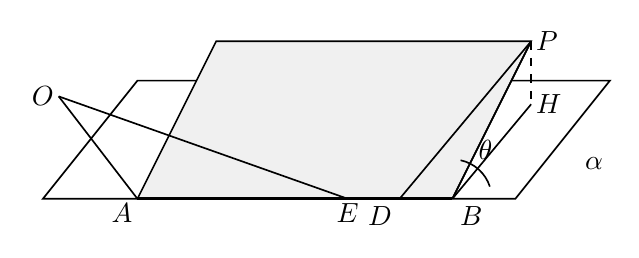
\begin{tikzpicture}[semithick, every node/.style={inner sep=1.5pt}]

  % 水平面 α
  \draw (0,0) -- (6,0) -- (7.2,1.5) -- (1.2,1.5) -- cycle;
  \node at (7.0,0.45) {$\alpha$};

  % 山坡面
  \coordinate (A) at (1.2,0);
  \coordinate (B) at (5.2,0);
  \coordinate (A2) at (2.2,2.0);
  \coordinate (B2) at (6.2,2.0);
  \fill[gray!12] (A) -- (B) -- (B2) -- (A2) -- cycle;
  \draw (A) -- (A2) -- (B2) -- (B);

  % 山脚公路 AB
  \draw[line width=1.1pt] (A) -- (B);

  % P、H、O
  \coordinate (P) at (6.2,2.0);
  \coordinate (H) at (6.2,1.2);
  \coordinate (O) at (0.2,1.3);
  \draw[dashed] (P) -- (H);
  \draw (H) -- (B);
  \draw (B) -- (P);
  \draw (O) -- (A);

  % D、E 及折线
  \coordinate (D) at (4.53,0);
  \coordinate (E) at (3.87,0);
  \draw (P) -- (D);
  \draw (E) -- (O);

  % 角 θ（BH 与 BP 之间）
  \draw (5.2,0) ++(18:0.5) arc[start angle=18, end angle=78, radius=0.5];
  \node at (5.62,0.62) {$\theta$};

  \node[left] at (O) {$O$};
  \node[below left] at (A) {$A$};
  \node[below right=1pt] at (B) {$B$};
  \node[below left=1pt] at (D) {$D$};
  \node[below] at (E) {$E$};
  \node[right] at (P) {$P$};
  \node[right] at (H) {$H$};
\end{tikzpicture}
\end{center}
\nopagebreak[4]
\Needspace{4\baselineskip}
\textbf{解析}

由 $PH\perp\alpha$，$PH=0.4$，$\sin\theta=\dfrac25$ 得 $PB=\dfrac{PH}{\sin\theta}=1$。

又 $PB\perp AB$，故对 $AB$ 上任意点 $D$ 有 $PD^2=PB^2+BD^2=1+BD^2$。设 $AD=d$，则 $BD=1.5-d$，山坡段造价为 $(PD^2+1)a=\left[2+(1.5-d)^2\right]a$。

\Needspace{5\baselineskip}
（1）折线 $PDAO$ 的造价

\nopagebreak[4]
\[C_1=a\left[2+(1.5-d)^2+\frac d2+\sqrt3\right],\qquad 0\leqslant d\leqslant1.5.\]

\Needspace{5\baselineskip}
对 $d$ 求导：

\nopagebreak[4]
\[C_1'=a\left[-2(1.5-d)+\frac12\right],\]

令 $C_1'=0$ 得 $d=\dfrac54$。且 $C_1''=2a>0$，故最小值在 $d=\dfrac54$ 处取得。

\Needspace{5\baselineskip}
此时 $BD=\dfrac14$，$PD^2=\dfrac{17}{16}$，

\nopagebreak[4]
\[C_{1,\min}=a\left[\frac{17}{16}+1+\frac58+\sqrt3\right]=a\left(\frac{43}{16}+\sqrt3\right).\]

\Needspace{5\baselineskip}
（2）设 $AE=e$（$0\leqslant e\leqslant d=\dfrac54$），则 $DE=d-e$。折线 $PDEO$ 的造价

\nopagebreak[4]
\[C_2=a\left[\frac{17}{16}+1+\frac{d-e}2+\sqrt{e^2+3}\right].\]

\Needspace{5\baselineskip}
记 $g(e)=\dfrac{d-e}2+\sqrt{e^2+3}$，则

\nopagebreak[4]
\[g'(e)=-\frac12+\frac{e}{\sqrt{e^2+3}}.\]

\Needspace{5\baselineskip}
令 $g'(e)=0$ 得 $e=1$。$g''(e)=\dfrac{3}{(e^2+3)^{3/2}}>0$，故 $e=1$ 为最小值点，此时 $AE=1$，$DE=\dfrac14$。

\nopagebreak[4]
\[C_{2,\min}=a\left[\frac{17}{16}+1+\frac18+2\right]=\frac{67a}{16}.\]

\Needspace{5\baselineskip}
（3）不存在。设 $AD=d$，$AE=e$（$0\leqslant e\leqslant d\leqslant1.5$），则折线 $PDEO$ 的造价为

\nopagebreak[4]
\[C(d,e)=a\left[2+(1.5-d)^2+\frac{d-e}2+\sqrt{e^2+3}\right].\]

\Needspace{5\baselineskip}
对固定的 $d$，关于 $e$ 的部分

\nopagebreak[4]
\[g(e)=\frac{d-e}2+\sqrt{e^2+3}\]

在 $e=\min\{1,d\}$ 处取最小值。当 $d\geqslant1$ 时 $e=1$；再对 $d$ 求导，$C(d,1)$ 在 $d=\dfrac54$ 处取最小值 $C\left(\dfrac54,1\right)=\dfrac{67a}{16}$。

\Needspace{5\baselineskip}
当 $d<1$ 时，$e=d$，此时

\nopagebreak[4]
\[C(d,d)=a\left[2+(1.5-d)^2+\sqrt{d^2+3}\right]\]

\Needspace{5\baselineskip}
关于 $d$ 单调递减（导数 $-2(1.5-d)+\dfrac{d}{\sqrt{d^2+3}}<0$），故

\nopagebreak[4]
\[C(d,d)>C(1,1)=a\left(2+\frac14+2\right)=\frac{17a}4>\frac{67a}{16}.\]

所以 $C(d,e)$ 在 $d=\dfrac54$，$e=1$ 处取唯一最小值。任意不同于此的点 $(D',E')$ 都使造价严格增大，故不存在满足要求的两个不同点。

\gkanswer{答案：（1）$AD=\dfrac54$ km，最小总造价 $a\left(\dfrac{43}{16}+\sqrt3\right)$ 万元；（2）$AE=1$ km，最小总造价 $\dfrac{67a}{16}$ 万元；（3）不存在，证明见解析。}

\end{answer}
\begin{answer}
\gksolhead{20}{}

\textbf{题目}：

已知双曲线 $x^2-y^2=2$ 的左、右焦点分别为 $F_1$，$F_2$，过点 $F_2$ 的动直线与双曲线相交于 $A$，$B$ 两点。

（1）若动点 $M$ 满足 $\overrightarrow{F_1M}=\overrightarrow{F_1A}+\overrightarrow{F_1B}+\overrightarrow{F_1O}$（其中 $O$ 为坐标原点），求点 $M$ 的轨迹方程；

（2）在 $x$ 轴上是否存在定点 $C$，使 $\overrightarrow{CA}\cdot\overrightarrow{CB}$ 为常数？若存在，求出点 $C$ 的坐标；若不存在，请说明理由。

\Needspace{4\baselineskip}
\textbf{解析}

双曲线 $x^2-y^2=2$ 中 $a^2=b^2=2$，$c=2$，故 $F_1(-2,0)$，$F_2(2,0)$。

\Needspace{5\baselineskip}
（1）由 $\overrightarrow{F_1M}=\overrightarrow{F_1A}+\overrightarrow{F_1B}+\overrightarrow{F_1O}$ 得

\nopagebreak[4]
\[M=A+B+O-2F_1=A+B+(4,0),\]

\Needspace{5\baselineskip}
故

\nopagebreak[4]
\[x_M=x_A+x_B+4,\qquad y_M=y_A+y_B.\]

\Needspace{5\baselineskip}
设过 $F_2$ 的直线为 $y=k(x-2)$，代入 $x^2-y^2=2$：

\nopagebreak[4]
\[(1-k^2)x^2+4k^2x-4k^2-2=0.\]

\Needspace{5\baselineskip}
由韦达定理

\nopagebreak[4]
\[x_A+x_B=\frac{4k^2}{k^2-1},\qquad y_A+y_B=k(x_A+x_B-4)=\frac{4k}{k^2-1}.\]

\Needspace{5\baselineskip}
于是

\nopagebreak[4]
\[x_M-4=\frac{4k^2}{k^2-1},\qquad y_M=\frac{4k}{k^2-1},\]

\Needspace{5\baselineskip}
两式相除得 $k=\dfrac{x_M-4}{y_M}$，代回 $y_M=\dfrac{4k}{k^2-1}$ 得

\nopagebreak[4]
\[(x_M-4)^2-y_M^2=4(x_M-4),\]

\Needspace{5\baselineskip}
即

\nopagebreak[4]
\[(x-6)^2-y^2=4.\]

\Needspace{5\baselineskip}
（2）设 $C(c,0)$，则

\nopagebreak[4]
\[\overrightarrow{CA}\cdot\overrightarrow{CB}=(x_A-c)(x_B-c)+y_Ay_B.\]

\Needspace{5\baselineskip}
由（1）的韦达定理，

\nopagebreak[4]
\[x_Ax_B=\frac{4k^2+2}{k^2-1},\qquad y_Ay_B=k^2(x_A-2)(x_B-2)=-\frac{2k^2}{k^2-1}.\]

\Needspace{5\baselineskip}
故

\nopagebreak[4]
\[\overrightarrow{CA}\cdot\overrightarrow{CB}
=\frac{4k^2+2-4ck^2-2k^2}{k^2-1}+c^2
=\frac{(2-4c)k^2+2}{k^2-1}+c^2.\]

\Needspace{5\baselineskip}
要使该式与 $k$ 无关，需 $2-4c=-2$，即 $c=1$。此时

\nopagebreak[4]
\[\overrightarrow{CA}\cdot\overrightarrow{CB}=-2+1=-1.\]

故存在定点 $C(1,0)$，使 $\overrightarrow{CA}\cdot\overrightarrow{CB}$ 恒为常数 $-1$。

\gkanswer{答案：（1）$(x-6)^2-y^2=4$；（2）存在 $C(1,0)$，$\overrightarrow{CA}\cdot\overrightarrow{CB}=-1$。}

\end{answer}
\begin{answer}
\gksolhead{21}{}

\textbf{题目}：

已知 $A_n(a_n,b_n)$（$n\in\mathbf N^*$）是曲线 $y=\mathrm e^x$ 上的点，$a_1=a$，$S_n$ 是数列 $\{a_n\}$ 的前 $n$ 项和，且满足 $S_n^2=3n^2a_n+S_{n-1}^2$，$a_n\neq0$，$n=2,3,4,\cdots$。

（1）证明：数列 $\left\{\dfrac{b_{n+2}}{b_n}\right\}$（$n\geqslant2$）是常数数列；

（2）确定 $a$ 的取值集合 $M$，使 $a\in M$ 时，数列 $\{a_n\}$ 是单调递增数列；

（3）证明：当 $a\in M$ 时，弦 $A_nA_{n+1}$（$n\in\mathbf N^*$）的斜率随 $n$ 单调递增。

\Needspace{4\baselineskip}
\textbf{解析}

\Needspace{5\baselineskip}
（1）由 $S_n^2-S_{n-1}^2=3n^2a_n$ 及 $S_n-S_{n-1}=a_n$，得

\nopagebreak[4]
\[a_n(S_n+S_{n-1})=3n^2a_n.\]

\Needspace{5\baselineskip}
$a_n\neq0$，故

\nopagebreak[4]
\[S_n+S_{n-1}=3n^2\qquad(n\geqslant2).\]

\Needspace{5\baselineskip}
于是对 $n\geqslant2$：

\nopagebreak[4]
\[a_{n+1}+a_n=(S_{n+1}+S_n)-(S_n+S_{n-1})=3(n+1)^2-3n^2=6n+3,\]

\nopagebreak[4]
\[a_{n+2}+a_{n+1}=3(n+2)^2-3(n+1)^2=6n+9.\]

\Needspace{5\baselineskip}
两式相减得

\nopagebreak[4]
\[a_{n+2}-a_n=6.\]

\Needspace{5\baselineskip}
又 $b_n=\mathrm e^{a_n}$，故

\nopagebreak[4]
\[\frac{b_{n+2}}{b_n}=\mathrm e^{a_{n+2}-a_n}=\mathrm e^6\]

为常数，即 $\left\{\dfrac{b_{n+2}}{b_n}\right\}$（$n\geqslant2$）是常数数列。

\Needspace{5\baselineskip}
（2）由 $S_2+S_1=12$ 得

\nopagebreak[4]
\[2a_1+a_2=12,\qquad a_2=12-2a.\]

\Needspace{5\baselineskip}
由 $a_3+a_2=15$ 得

\nopagebreak[4]
\[a_3=15-a_2=3+2a.\]

\Needspace{5\baselineskip}
又 $a_{n+2}=a_n+6$，故

\nopagebreak[4]
\[a_{2k}=6k+6-2a,\qquad a_{2k+1}=6k-3+2a.\]

\Needspace{5\baselineskip}
$\{a_n\}$ 单调递增等价于

\nopagebreak[4]
\[a_1<a_2,\quad a_2<a_3,\quad a_3<a_4,\quad\cdots\]

\Needspace{5\baselineskip}
其中

\nopagebreak[4]
\[a_1<a_2\ \Longleftrightarrow\ a<4,\]

\nopagebreak[4]
\[a_2<a_3\ \Longleftrightarrow\ 12-2a<3+2a\ \Longleftrightarrow\ a>\frac94,\]

\nopagebreak[4]
\[a_3<a_4\ \Longleftrightarrow\ 3+2a<18-2a\ \Longleftrightarrow\ a<\frac{15}4,\]

\Needspace{5\baselineskip}
且此后两类不等式分别重复上述两式。故

\nopagebreak[4]
\[M=\left(\frac94,\frac{15}4\right).\]

\Needspace{5\baselineskip}
（3）弦 $A_nA_{n+1}$ 的斜率

\nopagebreak[4]
\[k_n=\frac{\mathrm e^{a_{n+1}}-\mathrm e^{a_n}}{a_{n+1}-a_n}.\]

\Needspace{5\baselineskip}
记 $d_n=a_{n+1}-a_n>0$，$\varphi(t)=\dfrac{\mathrm e^t-1}{t}$，则

\nopagebreak[4]
\[k_n=\mathrm e^{a_n}\varphi(d_n),\qquad \varphi'(t)=\frac{\mathrm e^t(t-1)+1}{t^2}>0,\]

\Needspace{5\baselineskip}
且对 $t>0$ 有 $1<\varphi(t)<\mathrm e^t$。于是

\nopagebreak[4]
\[\frac{k_{n+1}}{k_n}=\mathrm e^{a_{n+1}-a_n}\cdot\frac{\varphi(d_{n+1})}{\varphi(d_n)}
=\mathrm e^{d_n}\cdot\frac{\varphi(d_{n+1})}{\varphi(d_n)}
>\mathrm e^{d_n}\cdot\frac1{\mathrm e^{d_n}}=1,\]

故 $k_{n+1}>k_n$，即弦 $A_nA_{n+1}$ 的斜率随 $n$ 单调递增。

\gkanswer{答案：（1）证明见解析；（2）$M=\left(\dfrac94,\dfrac{15}4\right)$；（3）证明见解析。}

\end{answer}